\documentclass[9pt]{beamer}
\usepackage[T1]{fontenc}
\usepackage[english]{babel}
\usepackage{xcolor}
\usepackage{amsfonts}
\usepackage{amsmath}
\usepackage{amssymb}
\usepackage{mathtools}
\usepackage{blkarray}
\usepackage{bm}
\usepackage{physics}
\usepackage{etoolbox}
\usepackage{eqparbox}
\usepackage{graphicx}

% Fonts
\renewcommand{\rmdefault}{ptm}
\renewcommand{\sfdefault}{phv}

% Spacing
\setlength\parindent{0pt}
\setlength\parskip{1ex plus 1ex minus 0.5ex}

% Basic notation
\DeclareMathOperator*{\argmax}{arg\,max}
\DeclareMathOperator*{\argmin}{arg\,min}
\renewcommand\d{\mathop{}\!\textnormal{\slshape d}}
\newcommand\eye{\mathop{}\!\mathbb{I}}
\newcommand\defined{\doteq}
\newcommand\upto{\stackrel{+}{=}}
\newcommand\without{\setminus}
\newcommand{\describe}[3][0pt]{\hspace*{.12em}\underbracket[0.5pt][1pt]{#2\hspace*{#1}}_\text{#3}}
\newcommand{\describel}[2]{\Shortunderstack[l]{$\underbracket[1pt][0pt]{#1}$ \raisebox{.8ex}{\scriptsize\rlap{#2}}}}
\newcommand{\changes}[1]{\underbracket[1pt][0pt]{#1}}

% Equation
\makeatletter
\newcommand{\removeParBefore}{\ifvmode\vspace*{-\baselineskip}\setlength{\parskip}{0ex}\fi}
\newcommand{\removeParAfter}{\@ifnextchar\par\@gobble\relax}
\newcommand{\eq}{\begingroup\removeParBefore\endlinechar=32 \eqinner}
\newcommand{\eqinner}[2][aligned]{\endlinechar=32%
\begin{gather}\begin{#1}#2\end{#1}\end{gather}\endgroup\removeParAfter}
\makeatother

% Density
\DeclareDocumentCommand{\p}{ D<>{p} D<>{} r() }{
\def\content{#3}\patchcmd{\content}{|}{\;#2\vert\;}{}{}
\ensuremath{#1 #2(\content #2)}}

% Probability
\DeclareDocumentCommand{\P}{ D<>{P} D<>{\big} r() }{
\def\content{#3}\patchcmd{\content}{|}{\;#2\vert\;}{}{}
\ensuremath{\operatorname{#1}#2(\content #2)}}

% Expectation
\DeclareDocumentCommand{\E}{ D<>{E} E{_}{{}} D<>{\big} r[] }{
\def\content{#4}\patchcmd{\content}{|}{\;#3\vert\;}{}{}
\ensuremath{\operatorname{#1}_{#2}#3[\content #3]}}

% Divergence
\DeclareDocumentCommand{\D}{ D<>{D} D<>{\big} r[] }{
\def\content{#3}\patchcmd{\content}{||}{\;#2\|\;}{}{}
\ensuremath{\operatorname{#1}\!#2[\content #2]}}

% Distributions
\NewDocumentCommand{\Nor}{ r() }{\P<Normal>](#1)}
\NewDocumentCommand{\Cat}{ r() }{\P<Cat>](#1)}
\NewDocumentCommand{\Bin}{ r() }{\P<Bin>](#1)}
\NewDocumentCommand{\Bet}{ r() }{\P<Beta>](#1)}
\NewDocumentCommand{\Ber}{ r() }{\P<Bernoulli>(#1)}
\NewDocumentCommand{\Dir}{ r() }{\P<Dir>(#1)}

% Information
\DeclareDocumentCommand{\KL}{ D<>{\big} r[] }{\D<KL><#1>[#2]}
\DeclareDocumentCommand{\H}{ D<>{\big} r[] }{\E<H><#1>[#2]}
\DeclareDocumentCommand{\I}{ D<>{\big} r[] }{\E<I><#1>[#2]}

% Symbols
\newcommand{\cmark}{\textcolor{green}{\ding{51}}}
\newcommand{\xmark}{\textcolor{red}{\ding{55}}}

% Shortcuts
\DeclareDocumentCommand{\lnpp}{ D<>{} r() }{
\ensuremath{\p<\ln p_\phi><#1>(#2)}}
\DeclareDocumentCommand{\pp}{ D<>{} r() }{
\ensuremath{\p<p_\phi><#1>(#2)}}
\DeclareDocumentCommand{\qp}{ D<>{} r() }{
\ensuremath{\p<q_\phi><#1>(#2)}}
\DeclareDocumentCommand{\SymLogNormal}{ D<>{} r() }{
\ensuremath{\p<\operatorname{SymLogNormal}><#1>(#2)}}
\newcommand{\sign}{\operatorname{sign}}
% \newcommand{\abs}{\operatorname{abs}}
\newcommand{\eps}{\epsilon}
% \newcommand{\erf}{\operatorname{erf}}
\newcommand{\fot}{\textstyle\frac{1}{2}}
\newcommand{\symlog}{\ensuremath{\operatorname{symlog}}}
\newcommand{\symexp}{\ensuremath{\operatorname{symexp}}}
\newcommand{\twohot}{\ensuremath{\operatorname{twohot}}}
\newcommand{\sg}{\ensuremath{\operatorname{sg}}}
\newcommand{\softmax}{\operatorname{softmax}}
\newcommand{\logsoftmax}{\operatorname{log\,softmax}}
\newcommand{\EMA}{\operatorname{EMA}}
\newcommand{\Per}{\operatorname{Per}}
\newcommand{\ema}{\operatorname{ema}}
\newcommand{\per}{\operatorname{per}}


\title{Transformer-based World Models Are Happy With 100k Interactions}
\date{April 30, 2025}

\definecolor{ObservColor}{HTML}{9FA8DA}
\definecolor{RepresColor}{HTML}{64B5F6}
\definecolor{ActionColor}{HTML}{EF5350}
\definecolor{RewardColor}{HTML}{9CCC65}
\definecolor{DiscntColor}{HTML}{CE93D8}
\definecolor{TransformerColor}{HTML}{FFC107}
\definecolor{HiddenColor}{HTML}{FF9800}
\definecolor{VoidColor}{HTML}{BDBDBD}

\begin{document}

\begin{frame}
    \titlepage
\end{frame}

\begin{frame}
    \frametitle{Reference}

    \bibliographystyle{plainnat}
    \bibliography{references}
\end{frame}

\begin{frame}
    
    \frametitle{Transformer-based World Model \citep{robine2023transformerbasedworldmodelshappy}}
    \begin{itemize}
        \item Transformer-based world model (TWM) generates meaningful, new experience
        \item Used to train a policy that outperforms previous model-free and model-based RL algorithms on Atari 100k benchmark
        \item Based on Transformer-XL architecture:
        \begin{itemize}
            \item Multiple self-attention layers with residual connections
            \item Causal masking prevents accessing future time steps
            \item Computationally efficient at inference time
            \item Uses relative positional encodings (removes dependence on absolute time steps)
        \end{itemize}
    \end{itemize}
\end{frame}

\begin{frame}
    \frametitle{Contributions}
    
    \begin{enumerate}
        \item New autoregressive world model based on Transformer-XL
        \begin{itemize}
            \item Model-free agent trained in latent imagination
            \item Transformer not needed at inference time % Computationally efficient policy
            % Contrast with related works requiring full world model during inference
        \end{itemize}
        
        \item Improved world model with reward feedback
        % Feeding back predicted rewards improves performance (shown in ablation study)
        
        \item Rewritten balanced KL divergence loss
        % Allows fine-tuning relative weight of entropy and cross-entropy terms
        
        \item New thresholded entropy loss
        \begin{itemize}
            \item Stabilizes policy entropy during training
            % Simplifies hyperparameter selection across different games
        \end{itemize}
        
        \item Effective sampling procedure for growing experience dataset
        % Balances training distribution toward latest experience
        % Efficacy demonstrated through ablation study
        
        \item Excellent results on Atari 100k benchmark
        \begin{itemize}
            \item Comparison with recent sample-efficient methods
            \item Reporting of empirical confidence intervals
        \end{itemize}
    \end{enumerate}
\end{frame}

\begin{frame}
    \frametitle{TWM Architecture}
    
    \begin{figure}[!b]
        \centering
        \resizebox{\textwidth}{!}{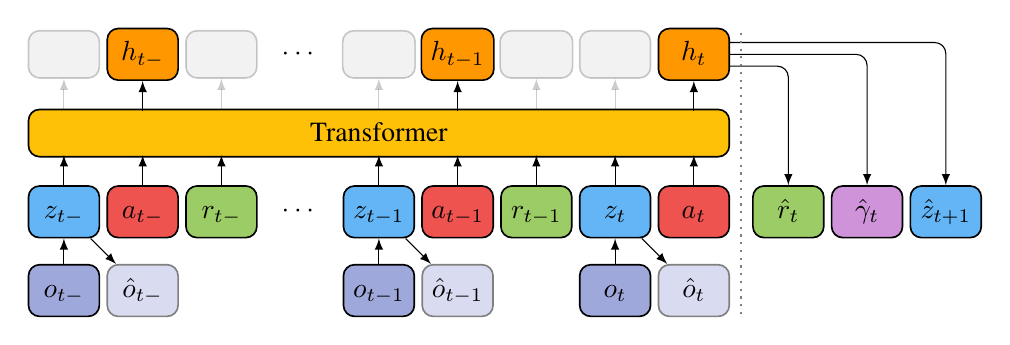
\begin{tikzpicture}
          \tikzset{Variable/.style={minimum width=0.9cm, minimum height=0.6cm, align=center, draw, semithick, rounded corners}}
          \tikzset{Observ/.style={Variable, black, fill=ObservColor}}
          \tikzset{Repres/.style={Variable, black, fill=RepresColor}}
          \tikzset{Action/.style={Variable, black, fill=ActionColor}}
          \tikzset{Reward/.style={Variable, black, fill=RewardColor}}
          \tikzset{Discnt/.style={Variable, black, fill=DiscntColor}}
          \tikzset{Transformer/.style={minimum height=0.6cm, align=center, text height=6pt, draw, semithick, rounded corners, black, fill=TransformerColor}}
          \tikzset{Hidden/.style={Variable, black, fill=HiddenColor}}
          \tikzset{Void/.style={Variable, black, fill=VoidColor, opacity=0.2}}
          \tikzset{Arrow/.style={->, >=latex, rounded corners}}
          \tikzset{VoidArrow/.style={->, >=latex, rounded corners, opacity=0.2}}
      
          \node[Observ] at (-7, -1) (otml) {$\strut{o}_{t-\historylength}$};
          \node[Repres] at (-7, 0) (ztml) {$\strut{z}_{t-\historylength}$};
          \node[Observ, draw=gray, fill=ObservColor!40!white] at (-6, -1) (recontml) {$\strut{\hat{o}}_{t-\historylength}$};
          \node[Void] at (-7, 2) (voidtml1) {\phantom{$h_{t-\historylength}$}};
          \node[Action] at (-6, 0) (atml) {$\strut{a}_{t-\historylength}$};
          \node[Hidden] at (-6, 2) (html) {$\strut{h}_{t-\historylength}$};
          \node[Reward] at (-5, 0) (rtml) {$\strut{r}_{t-\historylength}$};
          \node[Void] at (-5, 2) (voidtml2) {\phantom{$h_{t-\historylength}$}};
          \node at (-4, 0) (ellipsis1) {$\cdots$};
          \node at (-4, 2) (ellipsis2) {$\cdots$};
          \node[Observ] at (-3, -1) (otm1) {$\strut{o}_{t-1}$};
          \node[Repres] at (-3, 0) (ztm1) {$\strut{z}_{t-1}$};
          \node[Observ, draw=gray, fill=ObservColor!40!white] at (-2, -1) (recontm1) {$\strut{\hat{o}}_{t-1}$};
          \node[Void] at (-3, 2) (voidtm11) {\phantom{$h_{t-1}$}};
          \node[Action] at (-2, 0) (atm1) {$\strut{a}_{t-1}$};
          \node[Hidden] at (-2, 2) (htm1) {$\strut{h}_{t-1}$};
          \node[Reward] at (-1, 0) (rtm1) {$\strut{r}_{t-1}$};
          \node[Void] at (-1, 2) (voidtm12) {\phantom{$h_{t-1}$}};
          \node[Observ] at (0, -1) (ot) {$\strut{o}_t$};
          \node[Repres] at (0, 0) (zt) {$\strut{z}_t$};
          \node[Observ, draw=gray, fill=ObservColor!40!white] at (1, -1) (recont) {$\strut{\hat{o}}_t$};
          \node[Void] at (0, 2) (voidt) {\phantom{$h_t$}};
          \node[Action] at (1, 0) (at) {$\strut{a}_t$};
          \node[Hidden] at (1, 2) (ht) {$\strut{h}_t$};
          \node[Reward] at (2.2, 0) (rt) {$\strut{\hat{r}}_t$};
          \node[Discnt] at (3.2, 0) (dt) {$\strut\hat\gamma_t$};
          \node[Repres] at (4.2, 0) (ztp1) {$\strut{\hat{z}}_{t+1}$};
      
          \node[Transformer, minimum width=8.9cm] at (-3, 1) (transformer) {Transformer};
      
          \draw[Arrow] (otml.north) -- (ztml.south);
          \draw[Arrow] (ztml.north) -- ([yshift=0.38cm]ztml.north);
          \draw[Arrow] (atml.north) -- ([yshift=0.38cm]atml.north);
          \draw[Arrow] (rtml.north) -- ([yshift=0.38cm]rtml.north);
          \draw[Arrow] (otm1.north) -- (ztm1.south);
          \draw[Arrow] (ztm1.north) -- ([yshift=0.38cm]ztm1.north);
          \draw[Arrow] (atm1.north) -- ([yshift=0.38cm]atm1.north);
          \draw[Arrow] (rtm1.north) -- ([yshift=0.38cm]rtm1.north);
          \draw[Arrow] (ot.north) -- (zt.south);
          \draw[Arrow] (zt.north) -- ([yshift=0.38cm]zt.north);
          \draw[Arrow] (at.north) -- ([yshift=0.38cm]at.north);
      
          \draw[VoidArrow] ([yshift=-0.38cm]voidtml1.south) -- (voidtml1.south);
          \draw[Arrow] ([yshift=-0.38cm]html.south) -- (html.south);
          \draw[VoidArrow] ([yshift=-0.38cm]voidtml2.south) -- (voidtml2.south);
          \draw[VoidArrow] ([yshift=-0.38cm]voidtm11.south) -- (voidtm11.south);
          \draw[Arrow] ([yshift=-0.38cm]htm1.south) -- (htm1.south);
          \draw[VoidArrow] ([yshift=-0.38cm]voidtm12.south) -- (voidtm12.south);
          \draw[VoidArrow] ([yshift=-0.38cm]voidt.south) -- (voidt.south);
          \draw[Arrow] ([yshift=-0.38cm]ht.south) -- (ht.south);
          \draw[Arrow] ([yshift=-0.15cm]ht.east) -| (rt.north);
          \draw[Arrow] (ht.east) -| (dt.north);
          \draw[Arrow] ([yshift=0.15cm]ht.east) -| (ztp1.north);
      
          \draw[Arrow] (ztml) -- (recontml);
          \draw[Arrow] (ztm1) -- (recontm1);
          \draw[Arrow] (zt) -- (recont);
      
          \draw[gray, dotted, thick] (1.6, -1.3) -- (1.6, 2.3);
        \end{tikzpicture}}
        \vspace{-0.3cm}
        \caption{TWM architecture. Observations $o_{t-\ell:t}$ are encoded
        using a CNN. Linear embeddings of stochastic, discrete latent states
        $z_{t-\ell:t}$, actions $a_{t-\ell:t}$, and rewards $r_{t-\ell:t}$ are fed
        into a transformer, which computes a deterministic hidden state $h_t$ at each
        time step. Predictions of the reward $r_t$, discount factor $\gamma_t$, and
        next latent state $z_{t+1}$ are computed based on $h_t$ using MLPs.}
        \label{fig:transformer}
      \end{figure}
\end{frame}

\begin{frame}{World Model (1/3): Observation Model}
  \begin{itemize}
    \item The observation model is a VAE that compresses raw observations into compact latent states:
    \begin{align}
      \text{Encoder:} \quad z_t &\sim \obsprob(z_t \cond o_t) \\
      \text{Decoder:} \quad \hat{o}_t &\sim \obsprob(\hat{o}_t \cond z_t)
    \end{align}
    
    \item \textbf{Why a VAE?}
    \begin{itemize}
      \item \textbf{Compression:} Extracts essential features into a small latent representation
      \item \textbf{Stochasticity:} Sampling adds regularizing noise that prevents overfitting
    \end{itemize}
    
    \item \textbf{Discrete latents:} $z_t$ consists of 32 categorical variables with 32 categories
    \begin{itemize}
      \item This "discrete bottleneck" improves representation learning
      \item Forces clear distinctions between different latent states
    \end{itemize}
    
    \item \textbf{Frame stacking:} Although the VAE only processes $o_t$, each observation is already a stack of four recent frames, providing limited temporal context
  \end{itemize}
\end{frame}

\begin{frame}{World Model (2/3): Autoregressive Dynamics Model}
  The dynamics model predicts "what happens next" given everything it has produced so far:
  \begin{align}
    \text{Aggregation:} \quad h_t &= \dynfunc(z_{t-\historylength:t},a_{t-\historylength:t},r_{t-\historylength:t-1}) \\
    \text{Reward predictor:} \quad \hat{r}_t &\sim \dynprob(\hat{r}_t \cond h_t) \\
    \text{Discount predictor:} \quad \hat{\gamma}_t &\sim \dynprob(\hat{\gamma}_t \cond h_t) \\
    \text{Latent state predictor:} \quad \hat{z}_{t+1} &\sim \dynprob(\hat{z}_{t+1} \cond h_t)
  \end{align}
  
  \textbf{Transformer-XL Architecture:}
  \begin{itemize}
    \item \textbf{Causal masking:} Ensures attention only to past tokens
    \item \textbf{Recurrence cache:} Remembers information from arbitrarily far in the past
    \item \textbf{Relative positional encodings:} Remove dependence on absolute time indices
    \item \textbf{Input tokens:} Interleaved latent states, actions, and rewards for past $\ell$ steps
  \end{itemize}
\end{frame}

\begin{frame}{World Model (3/3): Why Fully Autoregressive Dynamics?}
  \textbf{Beneficial Properties:}
  \begin{itemize}
    \item \textbf{Autoregression:} Model directly sees its own past predictions
    \item \textbf{Parallel training:} Process all time steps at once (unlike RNNs)
    \item \textbf{Cached inference:} Only process newest tokens at test time
    \item \textbf{Long-term dependencies:} Capture far-past influences efficiently
  \end{itemize}
  
  \textbf{Advantages over traditional approaches:}
  \begin{itemize}
    \item \textbf{Richer dependencies:} Each past latent can be directly attended to
    \item \textbf{Robustness to prediction errors:} Model knows about past errors and can correct course
    \item \textbf{Adaptation to own noise:} Can react to randomness introduced by its own sampling
  \end{itemize}
  
  \textbf{Intuition:} By giving the dynamics model direct access to everything it has generated so far, it learns complex, self-aware temporal patterns. Transformers + recurrence provide scalability and memory, while autoregression enables adaptability to its own predictions.
\end{frame}

\begin{frame}{Loss Function (1/2): Observation Model Training}
  \textbf{Observation Model Loss:}
  \begin{equation}
    \loss_\obsparam^\text{Obs.} = \ev[\!][\bigg]{\,\sumt_{t=1}^T -\underbrace{\ln \obsprob(o_t \cond z_t)}_\text{decoder} - \underbrace{\entropycoef \ent{\obsprob(z_t \cond o_t)}}_\text{entropy regularizer} + \underbrace{\consistencycoef \ent{\obsprob(z_t \cond o_t),\dynprob(\hat{z}_t \cond h_{t-1})}}_\text{consistency}}\!
  \end{equation}
  , while \( H \) denotes the cross entropy loss function.
  
  \textbf{Components Explained:}
  \begin{itemize}
    \item \textbf{Decoder loss:} Teaches the model to reconstruct observations from latent states
    \item \textbf{Entropy regularizer:} Ensures latent space diversity by preventing collapse
    \item \textbf{Consistency loss:} Forces encoder to produce latents similar to what dynamics predicts
    \item Hyperparameters $\entropycoef, \consistencycoef$ let us balance exploration vs. consistency
  \end{itemize}
\end{frame}

\begin{frame}{Loss Function (2/2): Dynamics Model Training}
  \textbf{Dynamics Model Loss:}
  \begin{equation}
    \loss_\dynparam^\text{Dyn.} = \ev[\!][\bigg]{\,\sumt_{t=1}^T \underbrace{\ent{\obsprob(z_{t+1} \cond o_{t+1}),\dynprob(\hat{z}_{t+1} \cond h_t)}}_\text{latent state predictor} - \underbrace{\rewardcoef \ln \dynprob(r_t \cond h_t)}_\text{reward predictor} - \underbrace{\discountcoef \ln \dynprob(\gamma_t \cond h_t)}_\text{discount predictor}\,}\!
  \end{equation}
  , while \( H \) denotes the cross entropy loss function.
  
  \textbf{Components Explained:}
  \begin{itemize}
    \item \textbf{Latent state predictor:} Learns to predict the next latent state that the encoder would produce
    \item \textbf{Reward predictor:} Learns to anticipate rewards from current history
    \item \textbf{Discount predictor:} Learns to predict episode terminations ($\gamma_t = 0$ at episode end)
    \item Coefficients $\rewardcoef, \discountcoef$ balance importance of reward vs. termination prediction
  \end{itemize}
  
  \textbf{Key Benefits:}
  \begin{itemize}
    \item The balanced approach prevents either distribution from dominating
    \item Dynamics model can adapt to changing environments while maintaining stability
    \item Explicit cross-entropy terms give finer control than standard VAE training
    \item Self-supervised nature allows learning from unlabeled experience
  \end{itemize}
\end{frame}

\begin{frame}{Policy Learning (1/3): Actor-Critic on Imagined Trajectories}
  \textbf{Key Components:}
  \begin{itemize}
    \item \textbf{Imagined Rollouts:} Generate trajectories entirely inside the world model
    \item \textbf{Actor-Critic Architecture:}
      \begin{itemize}
        \item Actor: $\actor(a_t\mid \hat{z}_t)$ with parameters $\actorparam$
        \item Critic: $V_\criticparam(\hat{z}_t)$ with parameters $\criticparam$
      \end{itemize}
    \item \textbf{Advantage Estimation:} Use GAE with predicted discounts $\hat{\gamma}_t$
      \begin{equation}
        A_t = \sum_{k=0}^{\infty} \Bigl(\prod_{i=0}^{k-1}\hat\gamma_{t+i}\Bigr)\,r_{t+k} \;-\; V_\criticparam(\hat{z}_t)
      \end{equation}
    \item \textbf{Discount-Weighted Losses:} Multiply by cumulative product of $\hat{\gamma}$ to softly down-weight terms after predicted episode end
  \end{itemize}
\end{frame}

\begin{frame}{Policy Learning (2/3): Thresholded Entropy}
  \textbf{Thresholded Entropy Loss:}
  \begin{equation}
    \mathcal{L}^\text{Ent.}_\actorparam = \max\!\Bigl(0,\;\Gamma \;-\;\tfrac{H(\actor)}{\ln m}\Bigr)
  \end{equation}
  where $0 \leq \Gamma \leq 1$ is the threshold hyperparameter, $H(\actor)$ is the entropy of the policy, $m$ is the number of discrete actions, and $\ln(m)$ is the maximum possible entropy of the categorical action distribution.
  
  \textbf{Benefits:}
  \begin{itemize}
    \item \textbf{Normalized:} Entropy term lives in $[0,1]$ regardless of action-space size
    \item \textbf{Hinge effect:} No penalty when $H/\ln m \geq \Gamma$, linear penalty otherwise
    \item \textbf{Guaranteed exploration:} Maintains minimum exploration level without temperature schedules
  \end{itemize}
\end{frame}

\begin{frame}{Policy Learning (3/3): Efficient Inputs}

    The network must take some representation \( x_t \) of state. Options:

  \begin{table}
    \centering
    \begin{tabular}{cp{4cm}p{4cm}}
      \hline
      \textbf{Input} \( x_t \) & \textbf{Pros} & \textbf{Cons} \\
      \hline
      \( o_t \) & Stable—no drift & Heavy: requires conv-nets \\
      \( z_t \) & Light: small vectors & Drift between encodings \\
      \( [z_t,h_t] \) & Balance of stability/efficiency & Complex implementation \\
      \hline
    \end{tabular}
  \end{table}

  \textbf{Policy Input Choices:}
  \begin{itemize}
    \item \textbf{At inference (real env.):} $x_t = z_t$ with last 4 frames fed into VAE
    \item \textbf{At training (imagined rollouts):} $x_t = \hat{z}_t$ (model's predicted latents)
    \item \textbf{Efficiency gains:} Fast inference (single VAE encode per step) and fast training (small MLPs on $\hat{z}$)
  \end{itemize}
  
  \textbf{Summary:}
  \begin{itemize}
    \item Actor-critic leverages imagined futures with model's own $\hat{\gamma}_t$
    \item Thresholded entropy ensures fixed minimum exploration rate
    \item Lean inputs (compact discrete latent $z_t$) keep both training and inference efficient
  \end{itemize}
\end{frame}

\begin{frame}{Training (1/2): Overall Loop}
  \textbf{Three-phase training loop:}
  \begin{enumerate}
    \item \textbf{Collect real experience}
      \begin{itemize}
        \item Run policy $\pi_\theta$ in actual environment
        \item Record transitions $(o_t,\,a_t,\,r_t,\,d_t)$ where $d_t$ is done-flag
      \end{itemize}
    
    \item \textbf{Update World Model}
      \begin{itemize}
        \item Sample $\wmbatchsize$ short sequences of length $\historylength$ from dataset $\dataset$
        \item Compute observation loss $\loss^{\rm Obs.}_\obsparam$ and dynamics loss $\loss^{\rm Dyn.}_\dynparam$
        \item Update world-model parameters $(\obsparam,\dynparam)$
      \end{itemize}
    
    \item \textbf{Update Policy via Imagination}
      \begin{itemize}
        \item From same $\wmbatchsize \times \historylength$ observations, pick $\acbatchsize$ starting points
        \item "Roll out" each latent for $\achorizon$ steps inside world model:
          \begin{align*}
            \hat{z}_{t+1} &\sim p_\dynparam(\hat{z}_{t+1}\!\mid\!h_t) \\
            \hat{r}_t &\sim p_\dynparam(\hat{r}_t\!\mid\!h_t) \\
            \hat{\gamma}_t &\sim p_\dynparam(\hat{\gamma}_t\!\mid\!h_t) \\
            a_t &\sim \pi_\actorparam(a_t\!\mid\!\hat{z}_t)
          \end{align*}
        \item Compute actor-critic losses on imagined trajectories
        \item Update policy parameters $\actorparam$
      \end{itemize}
  \end{enumerate}
\end{frame}

\begin{frame}{Training (2/2): Balanced Dataset Sampling}
  \textbf{Problem:} Uniform sampling gives equal weight to early (poor) and recent (better) experience
  
  \textbf{Solution:} Softmax over "visitation counts"
  \begin{itemize}
    \item Track visitation count $v_i$ for each timestep $i$ used as sequence start
    \item Convert counts to sampling probabilities via softmax:
      \begin{equation}
        p_i = \frac{\exp\!\bigl(-v_i / \datasettemp\bigr)}
                   {\sum_{j=1}^{\datasetsize} \exp\!\bigl(-v_j / \datasettemp\bigr)}
      \end{equation}
  \end{itemize}
  
  \textbf{Temperature $\datasettemp$ controls recency bias:}
  \begin{itemize}
    \item $\datasettemp \to \infty$: Approaches uniform sampling
    \item Lower $\datasettemp$: Penalizes frequently-sampled steps, favors newer data
  \end{itemize}
  
  \textbf{Benefits:}
  \begin{itemize}
    \item Emphasizes fresh experience when data is scarce
    \item Prevents overfitting to early, untrained rollouts
    \item Can increase $\datasettemp$ as replay buffer grows for better stability
  \end{itemize}
\end{frame}

\begin{frame}{Experiment: Atari 100k}
    \begin{table}
        \centering
        \label{tab:results}
        \scriptsize
        \setlength{\tabcolsep}{4pt}
        \begin{adjustbox}{scale=0.93}
        \begin{tabular}{lrrrrrrrr}
          \toprule
          & & & \multicolumn{4}{c}{Model-free} & \multicolumn{2}{c}{Imagination} \\
          \cmidrule(lr){4-7}
          \cmidrule(lr){8-9}
          Game
          & Random
          & Human
          & DER
          & CURL
          & DrQ($\varepsilon$)
          & SPR
          & SimPLe
          & TWM (ours) \\
          \midrule
          Alien & 227.8 & 7127.7 & 802.3 & 711.0 & \textbf{865.2} & 841.9 & 616.9 & 674.6 \\
          Amidar & 5.8 & 1719.5 & 125.9 & 113.7 & 137.8 & \textbf{179.7} & 74.3 & 121.8 \\
          Assault & 222.4 & 742.0 & 561.5 & 500.9 & 579.6 & 565.6 & 527.2 & \textbf{682.6} \\
          Asterix & 210.0 & 8503.3 & 535.4 & 567.2 & 763.6 & 962.5 & \textbf{1128.3} & 1116.6 \\
          BankHeist & 14.2 & 753.1 & 185.5 & 65.3 & 232.9 & 345.4 & 34.2 & \textbf{466.7} \\
          BattleZone & 2360.0 & 37187.5 & 8977.0 & 8997.8 & 10165.3 & \textbf{14834.1} & 4031.2 & 5068.0 \\
          Boxing & 0.1 & 12.1 & -0.3 & 0.9 & 9.0 & 35.7 & 7.8 & \textbf{77.5} \\
          Breakout & 1.7 & 30.5 & 9.2 & 2.6 & 19.8 & 19.6 & 16.4 & \textbf{20.0} \\
          ChopperCommand & 811.0 & 7387.8 & 925.9 & 783.5 & 844.6 & 946.3 & 979.4 & \textbf{1697.4} \\
          CrazyClimber & 10780.5 & 35829.4 & 34508.6 & 9154.4 & 21539.0 & 36700.5 & 62583.6 & \textbf{71820.4} \\
          DemonAttack & 152.1 & 1971.0 & 627.6 & 646.5 & \textbf{1321.5} & 517.6 & 208.1 & 350.2 \\
          Freeway & 0.0 & 29.6 & 20.9 & \textbf{28.3} & 20.3 & 19.3 & 16.7 & 24.3 \\
          Frostbite & 65.2 & 4334.7 & 871.0 & 1226.5 & 1014.2 & 1170.7 & 236.9 & \textbf{1475.6} \\
          Gopher & 257.6 & 2412.5 & 467.0 & 400.9 & 621.6 & 660.6 & 596.8 & \textbf{1674.8} \\
          Hero & 1027.0 & 30826.4 & 6226.0 & 4987.7 & 4167.9 & 5858.6 & 2656.6 & \textbf{7254.0} \\
          Jamesbond & 29.0 & 302.8 & 275.7 & 331.0 & 349.1 & \textbf{366.5} & 100.5 & 362.4 \\
          Kangaroo & 52.0 & 3035.0 & 581.7 & 740.2 & 1088.4 & \textbf{3617.4} & 51.2 & 1240.0 \\
          Krull & 1598.0 & 2665.5 & 3256.9 & 3049.2 & 4402.1 & 3681.6 & 2204.8 & \textbf{6349.2} \\
          KungFuMaster & 258.5 & 22736.3 & 6580.1 & 8155.6 & 11467.4 & 14783.2 & 14862.5 & \textbf{24554.6} \\
          MsPacman & 307.3 & 6951.6 & 1187.4 & 1064.0 & 1218.1 & 1318.4 & 1480.0 & \textbf{1588.4} \\
          Pong & -20.7 & 14.6 & -9.7 & -18.5 & -9.1 & -5.4 & 12.8 & \textbf{18.8} \\
          PrivateEye & 24.9 & 69571.3 & 72.8 & 81.9 & 3.5 & 86.0 & 35.0 & \textbf{86.6} \\
          Qbert & 163.9 & 13455.0 & 1773.5 & 727.0 & 1810.7 & 866.3 & 1288.8 & \textbf{3330.8} \\
          RoadRunner & 11.5 & 7845.0 & 11843.4 & 5006.1 & 11211.4 & \textbf{12213.1} & 5640.6 & 9109.0 \\
          Seaquest & 68.4 & 42054.7 & 304.6 & 315.2 & 352.3 & 558.1 & 683.3 & \textbf{774.4} \\
          UpNDown & 533.4 & 11693.2 & 3075.0 & 2646.4 & 4324.5 & 10859.2 & 3350.3 & \textbf{15981.7} \\
          \midrule
          Normalized Mean & 0.000 & 1.000 & 0.350 & 0.261 & 0.465 & 0.616 & 0.332 & \textbf{0.956} \\
          Normalized Median & 0.000 & 1.000 & 0.189 & 0.092 & 0.313 & 0.396 & 0.134 & \textbf{0.505} \\
          \bottomrule
        \end{tabular}
        \end{adjustbox}
        \caption{Mean scores on Atari 100k benchmark with human normalized mean and median. Results averaged over $5$ runs per game, $100$ episodes per run. Bold indicates best scores.}
      \end{table}
\end{frame}

\begin{frame}{Analysis (1/2): Imagined Trajectories}
    \begin{figure}
        \captionsetup[subfigure]{aboveskip=3pt,belowskip=0pt}
      
        \begin{subfigure}{\textwidth}
          \includegraphics[width=\textwidth,trim=3247 60 5405 18,clip]{res/trajectories/boxing_1.pdf}
          \caption{Boxing. The player (white) presses \textit{fire}, hits the
            opponent, and gets a reward.}
          \vspace{0.1cm}
        \end{subfigure}
        \begin{subfigure}{\textwidth}
          \includegraphics[width=\textwidth,trim=4110 60 4540 18,clip]{res/trajectories/freeway_1.pdf}
          \caption{Freeway. The player moves up and bumps into a car. The world model
            correctly pushes the player down, although \textit{up} is still pressed.
            The movement of the cars is modeled correctly.}
          \label{fig:trajectory-freeway}
          \vspace{-0.2\baselineskip}
        \end{subfigure}
        \caption{Trajectories imagined by TWM. Above each frame they show the performed action and the produced reward.}
        \label{fig:trajectories}
      \end{figure}      
\end{frame}

\begin{frame}{Analysis (2/2): Attention Maps}
    \begin{figure}
        \centering
        \includegraphics[width=0.75\textwidth,trim=8 8 6 8]{res/attention_maps/assault_reward.pdf}
        \caption{Attention map of the learned transformer for the current hidden state
          $h$, computed on an imagined trajectory for the game Assault. The x-axis
          corresponds to the input sequence with the three modalities (states,
          actions, rewards), where the two rightmost columns are the current state and
          action. The y-axis corresponds to the layer of the transformer.}
        \label{fig:attention-map}
    \end{figure}
\end{frame}

\begin{frame}{Ablation Studies (1/2): Uniform Sampling}
    \begin{itemize}
        \item We evaluate the effectiveness of our balanced sampling procedure by comparing it with uniform sampling ($\datasettemp = \infty$ in Eqn. (11))
        \item Balanced sampling significantly improves performance across tested games
        \item Dynamics loss (Eqn. (8)) is lower with balanced sampling at training completion
        \item Possible explanation: uniform sampling causes the world model to overfit on early training data, leading to poor performance in later training stages
    \end{itemize}

    \begin{figure}
        \includegraphics[width=\textwidth]{res/uniform/hns.pdf}
        \caption{Comparison of balanced vs. uniform sampling across games. Human normalized scores during training show balanced sampling yields better performance, highlighting its importance.}
        \label{fig:uniform-sampling}
    \end{figure}
\end{frame}

\begin{frame}{Ablation Studies (2/2): No Rewards}

    \begin{itemize}
        \item Predicted rewards are fed back into the transformer
        \item They evaluate the impact of this design choice by comparing with a variant that doesn't use rewards as input
        \item Figure shows this feedback mechanism significantly increases performance in several games
        \item In some games, performance remains equivalent, likely because the world model can make correct predictions based solely on latent states and actions
    \end{itemize}

    \begin{figure}
        \includegraphics[width=\textwidth]{res/no_rewards/hns_1.pdf}
        \includegraphics[width=\textwidth]{res/no_rewards/hns_2.pdf}
        \caption{Effect of removing rewards from the input. Human normalized scores during training show conditioning on rewards significantly improves performance in some games, while others remain unaffected.}
        \label{fig:no-rewards}
    \end{figure}
\end{frame}


\end{document}